
\section{Color Palette Estimation}
\label{sec:cpe}

Im Folgenden wird eine Algorithmus zur Lösung des Teilproblems der Ermittlung der Farbobermenge $C_s$ gesucht. Hierzu findet eine Betrachtung von Typen vorhandener Algorithmen zur CPE statt. Abschließend wird ein geeigneter Algorithmus ausgewählt

\subsection{Überblick}

Grundlegend sind zwei Ansätze zur CPE zu unterscheiden:
\begin{enumerate}
    \item \textbf{Hisgoram-basiert}: Algorithmen, die nur auf dem Histogramm des Bildes arbeiten und somit die Positionsinformationen der Farben nicht beachten. Es handelt sich (bis auf Ausnahmen) um Clustering-Verfahren, die durch eine Partitionierung des Farbraums Gruppen ähnlicher Farben im Histogramm identifizieren.
    \item \textbf{Bildsegmentierungs-basiert}: Algorithmen, die durch eine Segmentierung des Bildes zunächst zusammenhängende Komponenten identifizieren und für diese dann repräsentative Farben identifizieren.
\end{enumerate}


Bildsegmentierungs-basierte Algorithmen berücksichtigen die menschlichen Wahrnehmungseigenschaften auf Komponentenebene, führen aber durch die zusätzliche Betrachtung der Positionsinformation eine weitere Komplexitätsebene ein \citep{colorthemes}.

\citet{categorization} treffen eine Kategorisierung der Histogramm-basierten Verfahren in \emph{hierarchisch} und \emph{iterativ}. Hierarchisch arbeitende Algorithmen zur CPE werden auch als \emph{Pre-Clustering Verfahren} bezeichnet, da sie vor dem Erreichen der (fest zu wählenden) Farbanzahl $n$ mit mehr bzw. weniger Farben starten. Sie basieren auf der statistischen Analyse der Verteilung der Bildfarben im Farbraum. In diese Kategorie fallen \emph{top-down} bzw. \emph{bottom-up} Clustering-Algorithmen. Zu den Top-Down Verfahren zählen die in der Vergangenheit populären Raumunterteilungs-Algorithmen wie z.B. Mediancut \citep{mediancut} oder Octree\citep{octree}. Sie Zerteilen den Farbraum sukzessiv in disjunkte Teilräume und unterstellen den Clustern dabei eine Würfelform. Ergebnis der Verarbeitung ist ein Dendogram, wobei die Blätter die Farben Farbpalette repräsentieren. Ein Schnitt des Dendograms entspricht einer Partitionierung des Raums, welche jedoch auch direkt durch die iterativ arbeitenden Algorithmen erreichbar ist \citep{acopa}. Diese Verfahren werden darum auch als \emph{partitionierend} \citep{acopa} oder auch \emph{Post-Clustering} \citep{categorization} bezeichnet. Sie starten bereits mit der erforderlichen Anzahl Farben $n$ und verbessern diese iterativ. Einige Methoden dieser Klasse verwenden den quadratischen Fehler, wie z.B. K-Means \citep{kmeans, kmeanshsi} oder Fuzzy C-Means \citep{fuccycmeans}. Andere analysieren das Histogramm auf dichte bzw. weniger dichte Regionen, wie z.B. Mean-Shift \citep{meanshift}. Eine detailliertere Vorstellung von Algorithmen zur CPE bietet \citep{categorization2}.

\begin{figure}[h]
\centering
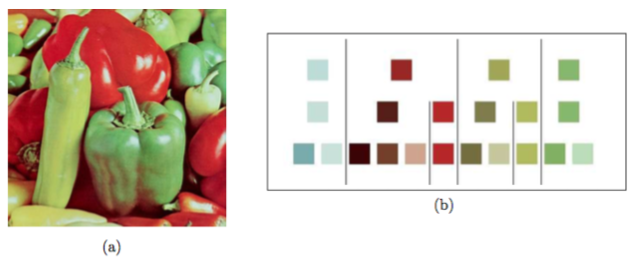
\includegraphics[width=0.48\textwidth]{img/peppers.png}
\caption{CPE Ergebnis von ACoPa. (a) Originalbild "Peppers" (b) Hierarchische Farbpalette. Die unterste Ebene zeigt die finalen Farben. (Quelle: \citep{acopa})}
\label{fig:peppers}
\end{figure}

\citet{acopa} kritisieren an den bisherigen Algorithmen, dass die Anzahl gesuchten Farben $n$ zuvor bekannt sein muss, dass die Ergebnisse abhängig von der Initialisierung sind und dass Farben kleiner Bilddetails im Sinne der Definition in Abschnitt \ref{sec:modellierung} nur unzureichend repräsentiert werden, wie im Paper experimentell nachgewiesen wird. Aus diesem Grund stellen sie den \textbf{Automatic Color Palette (ACoPa)} Algorithmus vor, welcher durch die Analyse von Spitzen des Histogramms im HSI Raums eine Farbpalette erstellt und dabei deren Größe selbstständig bestimmt. Der Algorithmus ermittelt dabei zunächst die grundlegenden Farbtöne (Hue) des Bildes und schlüsselt diese daraufhin sukzessive nach deren Sättigungen (Saturation) und Schattierungen (Intensity) auf. Abbildung \ref{fig:peppers} veranschaulicht exemplarisch die hierarchische Arbeitsweise, bei der in jeder Ebene zusätzliche Sättigungen und Schattierungen der enthaltenen roten und grünen Farbtöne gebildet werden.

\subsection*{Zusammenfassung und Wahl des Algorithmus zur CPE}

Der Algorithmus zur CPE soll eine Obermenge $C_s$ von Farben bilden, aus welcher im einem nachfolgenden Schritt eine Teilmenge von Farben $C$ entsprechend ihrer Eignung für bestimmte Oberflächenelemente ausgewählt werden. Analog dazu werden Farbpaletten in Styleguides als Obermenge von Farben beschrieben, aus welcher der Designer eine Untermenge von Farben für die konkrete Oberfläche auswählt. Bestimmte Styleguides erweitern dabei das Farbpalettenkonzept um Color Swatches, bei welchen Farbtöne in zusätzliche Schattierungen aufgefächert werden. Dadurch hat der der Designer eine größere Flexibilität beim Einsatz der Farbpalette.

Aus diesen Gründen wird der ACoPa Algorithmus von \citet{acopa} zur CPE gewählt. Da er Farbwerte automatisiert in verschiedenen Sättigungen und Schattierungen ermittelt, imitiert er die Farbdefinition in Form von Color Swatches in Styleguides. Durch seine parameterfreie Arbeitsweise ermittelt er selbstständig die Anzahl repräsentativer Farben im Bild. Dadurch wird automatisch die erforderliche Obermenge zur Bildung der finalen Farbpalette bereitgestellt, wenn das Bild ausreichend viele Farben enthält. Das erzwingen eines großen Farbpalette mit anderen Clusteringverfahren, z.B. über einen pauschal großen K Parameter bei K-Means, führt hingegen unter Umständen zu einer Partitionierung des Farbraums, die nicht der Clusterstruktur des Histogramms entspricht.

\section{ACoPa}

Im Folgenden wird die grundlegende Arbeitsweise des ACoPa Algorithmus nach \citet{acopa} vorgestellt. Dabei werden die Herausforderungen, die bei der Implementierung aufgetreten sind, besprochen. Abschließend werden exemplarisch Anwendungsergebnisse präsentiert.

\subsection{Konvertierung in den HSI-Raum}

\begin{figure*}
\centering
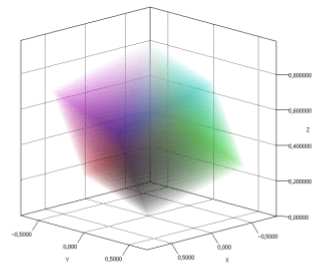
\includegraphics[width=1\textwidth]{img/hsi_conversion.png}
\caption{Gegenüberstellung von RGB zu HSI-Umrechungsergebnisse. (a.) Referenz-HSI Raum. (b.) Umrechnung nach \citep{acopa}. (c.) Umrechnung nach \citep{colorimage}.}
\label{fig:hsi_conversion}
\end{figure*}

Zunächst wird das Histogram in den HSI Farbraum $\{(h, s, i) \ | \ 0 \leq h < 360 \wedge 0 \leq s, i \leq 1\}$ übertragen. Die Intensität eines Farbtons wird dabei in Polarkoordinaten via $h$ und $s$ angegeben, während die maximal mögliche Sättigung wiederum von der Intensität $i$ abhängt. Zur Konvertierung vom RGB in HSI Raum wurden verschiedene Umrechnungsvorschriften erprobt. Die Umrechnung gemäß der ACoPa-Autoren lautet:

\begin{equation}
\begin{split}
I = \frac{R+G+B}{3} \\
S = \sqrt{(R-I)^2 + (G-I)^2 + (B-I)^2} \\  
H = \arccos{(\frac{(G-I)-(B-I)}{S\sqrt{2}})}
\end{split}
\label{eq:hsi_acopa}
\end{equation}

Die Umrechnung gemäß eines Lehrbuchs für Farbbild-Verarbeitung \citep{colorimage} lautet hingegen:

\begin{equation}
\begin{split}
I = \frac{R+G+B}{3} \\
S = 1 - \frac{\min{(R, G, B)}}{I} \\ 
H = \arccos{(\frac{\frac{1}{2}((R-G)+(R-B))}{\sqrt{(R-G)^2+(R-B)(G-B))}})}
\end{split}
\label{eq:hsi_colorimage}
\end{equation}

Abbildung \ref{fig:hsi_conversion} stellt die Umrechnungsergebnisse dem Referenz HSI Raum (R) gegenüber. Keine der Umrechnungsvorschriften führt zu einem Doppelkegel. Weder Formel \ref{eq:hsi_acopa} noch Formel \ref{eq:hsi_colorimage} projiziert die Farben mit 100\% Sättigung ($s = 1$) in eine Ebene. Formel \ref{eq:hsi_acopa} führt lediglich zu einer Drehung und Stauchung des RGB-Würfels, Formel \ref{eq:hsi_colorimage} führt zu einem nach unten geöffneten Kegel. Da schlussendlich keine Formel gefunden werden konnte, die zu einem korrekten Doppelkegel führt, wurde die Berechnung mit Formel \ref{eq:hsi_acopa} fortgeführt.

\subsection{Histogramm-Segmentierung}

Die Samples des Ausgangsbildes werden entlang der Hue-Werte sortiert. Das 1-dimensionale Hue-Histogram $h=(h_i)_{i = 1 \ldots b}$ mit b-Bins wird gebildet. Gesucht wird nun eine Sequenz $s = (s_i)_{i = 1 \ldots k}$ mit $1 = s_0 < s_1 < \ldots < s_k = b$, welche eine Segmentierung des Histograms darstellt. Das Intervall $[{s_i}, s_{i+1}]$ wird als Segment bezeichnet. Ziel ist, dass das Histogramm in den Bereichen $[h_{s_i}, \ldots,  h_{s_{i+1}}]$, eine \glqq annähernd unimodale Verteilung aufweist\grqq \citep{acopa}. Abbildung \ref{fig:unimodal} zeigt das Prinzip an verschiedenen Beispielen.

\begin{figure}[h]
\centering
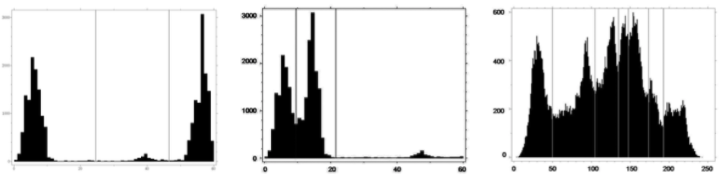
\includegraphics[width=0.48\textwidth]{img/unimodal.png}
\caption{Beispiele der Segmentierung eines Histograms in unimodale Abschnitte. (Quelle: \citep{acopa})}
\label{fig:unimodal}
\end{figure}

Das Histogramm ist offensichtlich in jedem Segment unimodal, wenn $s$ mit den Minima des Histograms initialisiert wird. Es wird nun versucht, Elemente aus $s$ zu entfernen, indem für $\forall i = 1 .. k$ überprüft wird, ob $h$ im Intervall $[h_{s_{i-1}}, \ldots,  h_{s_{i+1}}]$ die \glqq unimodale Hypothese\grqq  erfüllt. Anschaulich bedeutet das die Verschmelzung benachbarter Segmente, so dass das neu entstandene Segment nach wie vor \glqq annähernd unimodal ist\grqq. Hierfür stellen die Autoren in einer separaten Veröffentlichung \citep{ftc} einen parameterfreien statistischen Test vor, der $h$ im betrachteten Intervall mit einem Referenz-Histogramm $h^r$ vergleicht. $h^r$ ist in $[h^r_{s_{i-1}}, \ldots,  h^r_{s_{i+1}}]$ zunächst streng monoton wachsend und danach streng monoton fallend und damit in jedem Fall unimodal. Das Referenz-Histogramm wird aus dem Original-Histogramm $h$ durch Anwendung des Grenander-Operators gebildet. Die komplexen Details hierzu sind \citep{acopa, ftc} zu entnehmen. Da der parameterfreie Test verhältnismäßig aufwändig ist, wird in der eigenen Implementierung auf einen simplen T-Test zurückgegriffen. Dieser liefert ebenfalls befriedigende Ergebnisse, ist aber abhängig vom gewählten Signifikanzniveau.

Das Verfahren zur Histogramm-Segmentierung wird in \citep{ftc} als \textbf{Fine-to-Coarse (FTC) Segmentation Algorithm} zusammengefasst. Zunächst wird $s$ mit allen Minima des Histogramms initialisiert. Daraufhin werden so lange benachbarte Segmente durch Überprüfung der unimodalen Hypothese verschmolzen, bis keine Verschmelzung mehr möglich ist. Die Repräsentanten eines Segments werden durch Mittelung der Samples gebildet, die zum jeweiligen Segment gehören. Abbildung \ref{fig:h_segmentation} zeigt dies an einem Beispiel.

\begin{figure}[h]
\centering
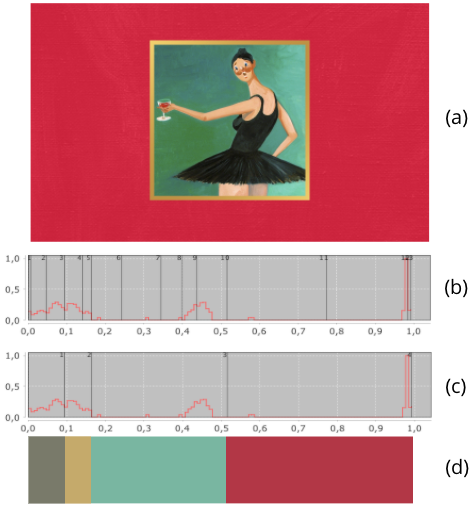
\includegraphics[width=0.48\textwidth]{img/h_segmentation.png}
\caption{Beispiel für eine Segmentierung des Hue-Histogramms. (a) Ausgangsbild, ein Albumcover  von Kanye West. (b) Hue-Histogram (normalisiert), mit allen Minima als initiale Segmentierung. (c) Segmentierung nach Anwendung des FTC Algorithmus. (d) Farbmittelpunkte entsprechend der Samples der jeweiligen Segmente.}
\label{fig:h_segmentation}
\end{figure}

\subsection{Bildung der hierarchischen Farbpalette}

Der ACoPa Algorithmus besteht aus einer hierarchischen Anwendung der Histogram-Segmentierung. Dabei wird zuerst der $h$-, danach der $s$- und abschließend der $i$- Kanal segmentiert. Dabei werden in jedem Schritt die Samples der entstandenen Segmente separiert und die Histogramme der nächsten Ebene getrennt berechnet. Das Ergebnis ist eine hierarchische Farbpalette. Abbildung \ref{fig:palette} zeigt dies am Beispiel der Covers aus Abbildung \ref{fig:h_segmentation}. Auf oberster Ebene (h) wurden die grundsätzlichen Farbtöne des Bildes identifiziert. Auf der zweiten Ebene werden die Farbtöne jeweils in unterschiedliche Sättigungen aufgeteilt, wenn nötig. Auf der dritten Ebene (i) werden von den Sättigungen zusätzlich Helligkeitsabstufungen gebildet.

Die letzte Ebene (i) bildet die Obermenge der Farben $C_s$ für die weitere Verarbeitung. \citet{acopa} empfehlen zusätzlich, die erhaltenen Farben als Startpunkte für den K-Means Algorithmus zu verwenden. Abbildung \ref{fig:palette} (b) zeigt, wie sich die Farben durch K-Means geändert haben. Es ist zu einem späteren Zeitpunkt zu entschieden, welche der beiden Paletten für die weitere Verarbeitung geeigneter ist.

\begin{figure}[h]
\centering
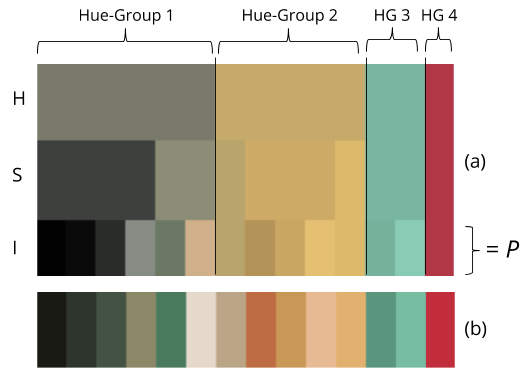
\includegraphics[width=0.48\textwidth]{img/palette.png}
\caption{(a) Hierarchische Farbpalette des Covers aus Abbildung \ref{fig:h_segmentation}. (b) Farbpalette nach Anwendung von K-Means.}
\label{fig:palette}
\end{figure}

